Throughout this chapter, let \(\mathcal{C}\) be a fixed locally small category. A weighted type graph is an object \(T\) in \(\mathcal{C}\), called the type graph, equipped with a distinguished family of morphisms into \(T\), each endowed with a weight. 
A \enquote{type graph} is an object, following the terminology from the previous work by Bruggink~\cite{bruggink2014termination}.
 Given a weighted type graph and any object \(X\) in \(\mathcal{C}\), we interpret \(X\) as \(\operatorname{Hom}(X,T)\). The distinguished morphisms determine weight assignments on the elements of \(\operatorname{Hom}(X,T)\); the weight of \(X\) is then defined as the sum of the weights of the morphisms in \(\operatorname{Hom}(X,T)\). These assignments provide a basis for comparing objects of \(\mathcal{C}\) according to their weights.

\begin{definition}[\cite{endrullis2024generalized_arxiv_v2}]
    \label{wf:def:weighted_type_graph}
    A \textbf{weighted type graph} is a tuple~\(\mathcal{T} \mathop{=} (T, \mathbb{E}, \mathcal{S}, w)\) where
    \begin{itemize} 
        \item \(T\) is an object of $\mathcal{C}$, called \textbf{type graph},
        \item \(\mathbb{E}\) is a set of morphisms in $\mathcal{C}$ with codomain $T$, and the elements of \(\mathbb{E}\) are called \textbf{morphism-rulers},
        \item \(\mathcal{S}=(S, \mathop{\oplus}, \mathop{\odot}, 0, 1)\) is a commutative semiring,
        \item \(w : \mathbb{E} \mathop{\to} S \mathop{\setminus} \{0\}\) is a weight function such that for all $e \mathop{\in} \mathbb{E}, w(e) \mathop{\geq} 1$,
    \end{itemize}
    % The weighted type graph \(\mathcal{T}\) is \textbf{finitary} if for every \( (e :X \mathop{\to} T) \mathop{\in} \mathbb{E}\) and every object \(G\), \(\operatorname{Hom}(X, G)\) and \(\operatorname{Hom}(G, T)\) are finite sets.
    such that for every \( (e :X \mathop{\to} T) \mathop{\in} \mathbb{E}\) and every object \(G\), \(\operatorname{Hom}(X, G)\) and \(\operatorname{Hom}(G, T)\) are finite sets.
\end{definition}

\begin{example}
    \label{wf:example:weighted_type_graph}
     Consider the weighted type graph $\mathcal{T} \mathop{=} (T, \mathbb{E}, \mathcal{S}, w)$ where
    \begin{itemize}
        \item $T$ is the labeled graph shown below:
        % in Figure~\ref{fig:weighted_type_graph_instance_dfjlsjl},
        % \begin{figure}[H]
        %     \centering
        \begin{center}
            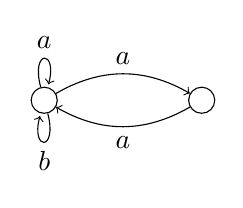
\begin{tikzpicture}
                    \graphbox{}{0mm}{0mm}{32mm}{28mm}{-10mm}{-14mm}{
                        \node[draw,circle] (1) at (0,0) {};
                        \node[draw,circle] (2) at (2,0) {};
                        \draw[->] (1) edge[loop above] node[midway, above] {$a$} (1) ;
                        \draw[->] (1) edge[loop below] node[midway, below] {$b$} (1) ;
                        \draw[->] (1) edge[bend left] node[midway, above] {$a$}  (2)  ;
                        \draw[->] (2) edge[bend left] node[midway, below] {$a$} (1)   ;
                    }
                \end{tikzpicture}
        \end{center}
            %     \caption{}
            %     \label{fig:weighted_type_graph_instance_dfjlsjl}
            % \end{figure}
        \item $\mathcal{S}$ is the natural arithmetic semiring $(\mathbb{N}, +_\mathbb{N}, *_\mathbb{N}, 0_\mathbb{N}, 1_\mathbb{N}, <_\mathbb{N},\leq_\mathbb{N})$,
        \item $\mathbb{E}$ consists of 4 morphism-rulers $e_{11a}, e_{12a}, e_{21a}, e_{11b}$ shown
            below:
        %  in Figure~\ref{fig:morphism_ruler__dfjsdlfjsadl}.
            % \begin{figure}[H]
            %    \centering
            \begin{center}
        \resizebox{0.69\textwidth}{!}{
            \begin{tikzpicture}
            \graphbox{\( K \)}{-50mm}{0mm}{40mm}{30mm}{2mm}{-6mm}{
                \coordinate (o) at (0mm,-10mm); 
                    \node[draw,circle] (l1) at ($(o)+(-10mm,0mm)$) {$1$};
                    \node[draw,circle] (l2) at ($(l1)+(2,0)$) {$2$};
                    \draw[->] (l1) -- (l2) node[midway,above] {$a$};
                } 
                \graphbox{$T$}{0mm}{0mm}{40mm}{30mm}{-10mm}{-15mm}{
                    \node[draw,circle] (1) at (0,0) {$1\ 2$};
                    \node[draw,circle] (2) at (2,0) {};
                    \draw[->] (1) edge[loop above] node[midway, above] {$a$} (1) ;
                    \draw[->] (1) edge[loop below] node[midway, below] {$b$} (1) ;
                    \draw[->] (1) edge[bend left] node[midway, above] {$a$}  (2)  ;
                    \draw[->] (2) edge[bend left] node[midway, below] {$a$} (1)   ;
                }
                \node () at (-5mm,-15mm) {$\overset{e_{11a}}{\to}$};
            \end{tikzpicture}
            } 

            \resizebox{0.69\textwidth}{!}{
            \begin{tikzpicture}
                \graphbox{\( K \)}{-50mm}{0mm}{40mm}{28mm}{2mm}{-6mm}{
                    \coordinate (o) at (0mm,-10mm); 
                    \node[draw,circle] (l1) at ($(o)+(-10mm,0mm)$) {$1$};
                    \node[draw,circle] (l2) at ($(l1)+(2,0)$) {$2$};
                    \draw[->] (l1) -- (l2) node[midway,above] {$b$};
                } 
                \graphbox{$T$}{0mm}{0mm}{40mm}{28mm}{-10mm}{-15mm}{
                    \node[draw,circle] (1) at (0,0) {$1\ 2$};
                    \node[draw,circle] (2) at (2,0) {};
                    \draw[->] (1) edge[loop above] node[midway, above] {$a$} (1) ;
                    \draw[->] (1) edge[loop below] node[midway, below] {$b$} (1) ;
                    \draw[->] (1) edge[bend left] node[midway, above] {$a$}  (2)  ;
                    \draw[->] (2) edge[bend left] node[midway, below] {$a$} (1)   ;
                }
                \node () at (-5mm,-15mm) {$\overset{e_{11b}}{\to}$};
            \end{tikzpicture}
            }

            \resizebox{0.69\textwidth}{!}{
                \begin{tikzpicture}
                    \graphbox{\( K \)}{-50mm}{0mm}{40mm}{28mm}{2mm}{-6mm}{
                        \coordinate (o) at (0mm,-10mm); 
                        \node[draw,circle] (l1) at ($(o)+(-10mm,0mm)$) {$1$};
                        \node[draw,circle] (l2) at ($(l1)+(2,0)$) {$2$};
                        \draw[->] (l1) -- (l2) node[midway,above] {$a$};
                    } 
                    \graphbox{$T$}{0mm}{0mm}{40mm}{26mm}{-10mm}{-15mm}{
                        \node[draw,circle] (1) at (0,0) {$1$};
                        \node[draw,circle] (2) at (2,0) {$2$};
                        \draw[->] (1) edge[loop above] node[midway, above] {$a$} (1) ;
                        \draw[->] (1) edge[loop below] node[midway, below] {$b$} (1) ;
                        \draw[->] (1) edge[bend left] node[midway, above] {$a$}  (2)  ;
                        \draw[->] (2) edge[bend left] node[midway, below] {$a$} (1)   ;
                    }
                    \node () at (-5mm,-15mm) {$\overset{e_{12a}}{\to}$};
                \end{tikzpicture}
            }

            \resizebox{0.69\textwidth}{!}{
            \begin{tikzpicture}
                \graphbox{\( K \)}{-50mm}{0mm}{40mm}{28mm}{2mm}{-6mm}{
                    \coordinate (o) at (0mm,-10mm); 
                    \node[draw,circle] (l1) at ($(o)+(-10mm,0mm)$) {$1$};
                    \node[draw,circle] (l2) at ($(l1)+(2,0)$) {$2$};
                    \draw[->] (l1) -- (l2) node[midway,above] {$a$};
                } 
                \graphbox{$T$}{0mm}{0mm}{40mm}{28mm}{-10mm}{-15mm}{
                    \node[draw,circle] (1) at (0,0) {2};
                    \node[draw,circle] (2) at (2,0) {1};
                    \draw[->] (1) edge[loop above] node[midway, above] {$a$} (1) ;
                    \draw[->] (1) edge[loop below] node[midway, below] {$b$} (1) ;
                    \draw[->] (1) edge[bend left] node[midway, above] {$a$}  (2)  ;
                    \draw[->] (2) edge[bend left] node[midway, below] {$a$} (1)   ;
                }
                \node () at (-5mm,-15mm) {$\overset{e_{21a}}{\to}$};
            \end{tikzpicture}
            }
        \end{center}
            %     \caption{}
            %     \label{fig:morphism_ruler__dfjsdlfjsadl}
            % \end{figure}
        \item $w(e) \mathop{=} 1_\mathbb{N}$ for all $e \mathop{\in} \mathbb{E}$.
         \end{itemize}
    %  with 
% $\mathbb{E}=\{e_{11a},e_{12a},e_{21a},e_{11b}\}$ as the set of morphism-rulers where 
%      $e_{uvl}$, for all edge from $u$ to $v$ labeled by $l$, has domain 
%      \tikz[baseline=-0.5ex]{
%         \node[draw,circle] (x) at (0,0) {};
%         \node[draw,circle] (y) at (1,0) {};
%         \draw[->] (x) -- (y) node[midway, above] {$l$};
%     } and image 
%     \begin{tikzpicture}[baseline=-2mm]
%         \node[draw, circle] (x) at (0,0) {$\mathrm{u}$};
%         \node[draw, circle] (y) at (1,0) {$\mathrm{v}$};
%         \draw[->]  (x) -- (y) node [midway,above] {$l$};
%     \end{tikzpicture} in the graph $T$,
    % and $w(e) \mathop{=} 1_\mathbb{N}$ for all $e \mathop{\in} \mathbb{E}$, is visualized in Figure~\ref{fig:weighted_type_graph_instance}. 
    To improve readability, this weighted type graph will visualized as shown below, where a label $l$ with superscript $n$ on an edge means that there is a morphism-ruler with weight $n$ from \raisebox{2pt}{
            \scalebox{0.7}{\tikz[baseline=-0.5ex]{
            \node [draw,circle] (x) at (0,0) {};
            \node[draw,circle] (y) at (1,0) {};
            \draw[->] (x)--(y) node[midway, above] {$l$};
        }}} to this edge in $\mathbb{E}$.
    % \begin{figure}[H]
    %     \centering
    \begin{center}
        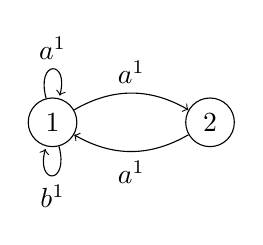
\begin{tikzpicture}
            \graphbox{}{0mm}{0mm}{32mm}{28mm}{-10mm}{-14mm}{
                \node[draw,circle] (1) at (0,0) {1};
                \node[draw,circle] (2) at (2,0) {2};
                \draw[->] (1) edge[loop above] node[midway, above] {$a^{1}$} (1) ;
                \draw[->] (1) edge[loop below] node[midway, below] {$b^{1}$} (1) ;
                \draw[->] (1) edge[bend left] node[midway, above] {$a^{1}$}  (2)  ;
                \draw[->] (2) edge[bend left] node[midway, below] {$a^{1}$} (1)   ;
            }
        \end{tikzpicture}
    \end{center}
    %     \caption{}
    %     \label{fig:weighted_type_graph_instance}
    % \end{figure}
\end{example}